\documentclass{standalone}
\usepackage{tikz}
\usepackage{ctex,siunitx}
\setCJKmainfont{Noto Serif CJK SC}
\usepackage{tkz-euclide}
\usepackage{amsmath}
\usetikzlibrary{patterns, calc,3d}
\usetikzlibrary {decorations.pathmorphing,decorations.pathreplacing,decorations.shapes}
\begin{document}
\small
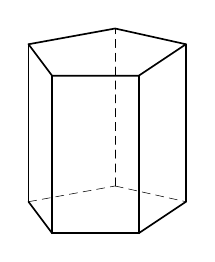
\begin{tikzpicture}[>=latex,scale=1.0]
  \tkzDefPoints{0/0/A,0.3/-0.4/B,1.4/-0.4/C,2/0/D,1.1/0.2/E,0/2.0/A'}
  \tkzDefPointsBy[translation=from A to A'](B,C,D,E){B',C',D',E'}
  \tkzDrawPolygon[semithick](A',B',C',D',E')
  \tkzDrawSegments[densely dashed](A,E E,D E,E')
  \tkzDrawSegments[semithick](A,A' B,B' C,C' D,D' A,B B,C C,D)
\end{tikzpicture}
\end{document}